% -----------------------------------------------------------------------------
% DEXPI Beamer Theme
% -----------------------------------------------------------------------------
% Copyright (c) 2026 DEXPI e.V.
%
% This work is licensed under the Creative Commons Attribution-ShareAlike 4.0
% International License (CC BY-SA 4.0).
%
% You are free to:
%   - Share: copy and redistribute the material in any medium or format
%   - Adapt: remix, transform, and build upon the material for any purpose
%
% Under the following terms:
%   - Attribution: You must give appropriate credit to DEXPI e.V.,
%     provide a link to the license, and indicate if changes were made.
%   - ShareAlike: If you remix, transform, or build upon the material,
%     you must distribute your contributions under the same license.
%
% Full license text:
%   https://creativecommons.org/licenses/by-sa/4.0/
%
%  Author: Michael Wiedau
% -----------------------------------------------------------------------------

%----------------------------------------------------------------------------------------
%    PACKAGES AND THEMES
%----------------------------------------------------------------------------------------

\documentclass[aspectratio=169,xcolor=dvipsnames]{beamer}
\usetheme{DEXPI}

\usepackage{hyperref}
\usepackage{graphicx}
\usepackage{booktabs}
\usepackage{pgfgantt}
\usepackage[portuguese]{babel}


\usepackage{tikz}
\usepackage{circuitikz}
\usetikzlibrary{shapes.geometric,calc,positioning,decorations.pathreplacing}
\usepackage{pgfplots}
\pgfplotsset{compat=1.10}
\usepackage{color}

\newcommand{\hrefcol}[2]{\textcolor{cyan}{\href{#1}{#2}}}



% adicionar o numero na lista final da apresentação
\setbeamertemplate{bibliography item}{\insertbiblabel}


%----------------------------------------------------------------------------------------
%    TITLE PAGE
%----------------------------------------------------------------------------------------

\title{Vazamento}
%\subtitle{Licensed under CC-BY-SA}

\author{%
Thiago Abreu \and Evandro Rocha  \\%
Caio Lacoste \and Pedro Ivo %
}
\date{\today}
\institute{Laboratório de Processamento de Sinais (LPS)}


%----------------------------------------------------------------------------------------
%    PRESENTATION SLIDES
%----------------------------------------------------------------------------------------

\begin{document}
\begin{frame}[plain]
    \titlepage
\end{frame}

\begin{frame}{Conteúdo da Apresentação}
    % Throughout your presentation, if you choose to use \section{} and \subsection{} commands, these will automatically be printed on this slide as an overview of your presentation
    \tableofcontents
\end{frame}

\section{Evolução do Conceito de GD}


\begin{frame}[plain]
    \vfill
    \centering
    {\Large\textcolor{dexpiBlue}{\textbf{Seção 1}}}\\[0.8em]
    {\LARGE\textbf{Evolução do Conceito  de Gêmeo Digital}}\\[0.6em]
    \vfill
\end{frame}

\begin{frame}{Evolução do Conceito  de Gêmeo Digital}
Artigo: What is a Digital Twin anyway? Deriving the definition for the built environment from over 15,000 scientific publications (2025)

    \begin{figure}
        \centering
        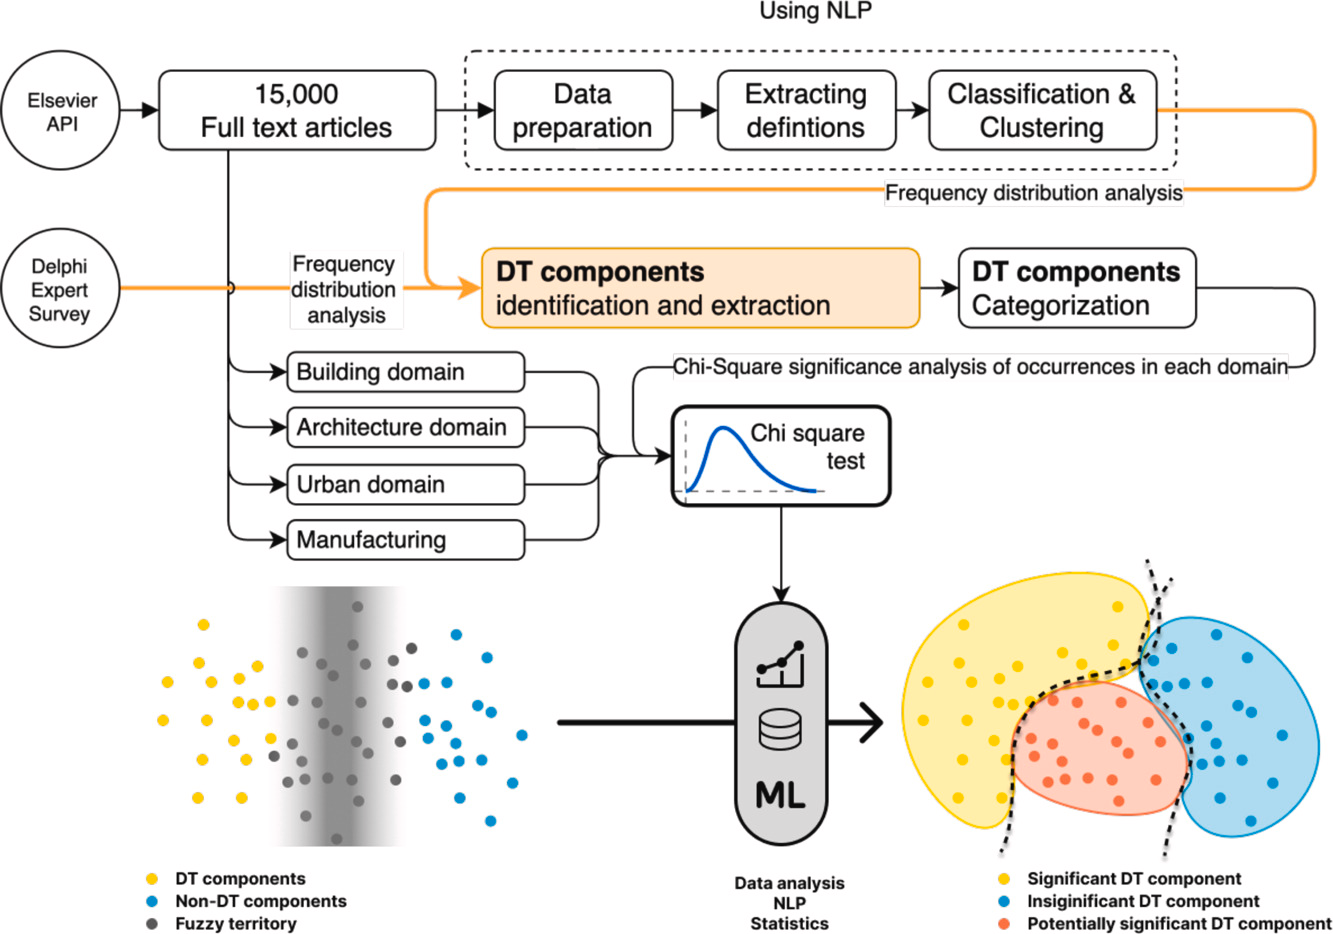
\includegraphics[width=0.9\linewidth, height=5.5cm]{figures/NLP_derived_definition.png}
    \end{figure}
\end{frame}

\begin{frame}{Evolução do Conceito  de Gêmeo Digital}

A definição de GD ainda está se consolidando e varia significativamente entre indústrias.

GDs em geral se separam entre dois grupos:
\begin{itemize}
    \item High-Performance Real Time (HPRT): Caracterizado por componentes dinâmicos, operando em tempo real e orientados por \textit{big data}. São comumente utilizados na manufatura, no setor aeroespacial e em veículos autônomos.
    \item Long-Term Decision Support (LTDS): Adequado para aplicações que exigem planejamento e gestão de longo prazo, como o planejamento urbano e a gestão de edificações.
\end{itemize}
\end{frame}

\begin{frame}{Evolução do Conceito de Gêmeo Digital}
Artigo: Digital Twin Technology: A Comprehensive Review of Modeling, Applications, Challenges and Future Directions in Complex System Integration (2026).

\begin{itemize}
    \item DT refere-se a uma representação digital em tempo real e orientada por dados de um sistema físico, projetada para apoiar o monitoramento, a simulação e a tomada de decisões preditivas. 
    \item  Idealmente, todos os detalhes que podem ser obtidos a partir do estudo do sistema físico também podem ser encontrados em seu DT.
    \item Os dados desempenham um papel crucial na eficácia de um DT.
    \item A versão digital utiliza modelos de engenharia integrados e IA para analisar esses dados. 
\end{itemize}
\end{frame}

\begin{frame}{Evolução do Conceito de Gêmeo Digital}
    \begin{itemize}
        \item Um DT difere fundamentalmente de uma “sombra digital” por integrar dados do mundo físico a modelos virtuais. Essa abordagem permite que a DT processe um volume maior de dados do que as “sombras digitais”, resultando em uma representação mais abrangente e dinâmica do objeto ou sistema monitorado.
        \item  Ao integrar dados em tempo real com modelos virtuais avançados, as tecnologias de DT superam as limitações das “sombras digitais”, consolidando-se como ferramentas indispensáveis para setores que exigem alta capacidade preditiva, gestão eficiente de recursos e desempenho ideal.
    \end{itemize}
\end{frame}

\section{Evolução da Arquitetura}

\begin{frame}[plain]
    \vfill
    \centering
    {\Large\textcolor{dexpiBlue}{\textbf{Seção 2}}}\\[0.8em]
    {\LARGE\textbf{Evolução da Arquitetura}}\\[0.6em]
    \vfill
\end{frame}

\begin{frame}{Arquitetura da Solução de GD}

    \begin{figure}
        \centering
        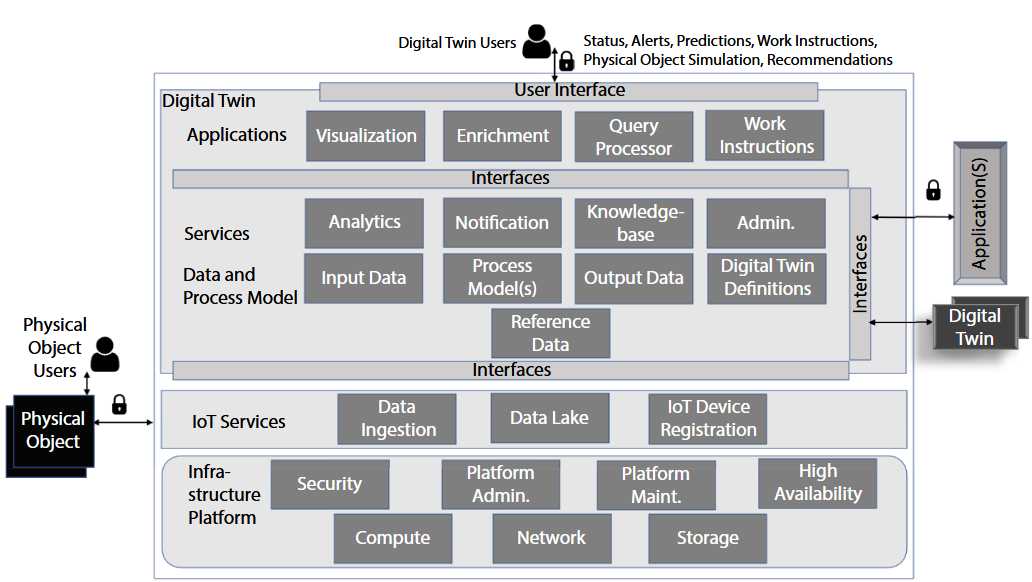
\includegraphics[width=0.8\linewidth]{figures/GD_arch.png}
    \end{figure}
\end{frame}

\begin{frame}{Evolução de Arquitetura de GD}
Artigo: A Survey on Digital Twin Networks: Architecture,
Technologies, Applications, and Open Issues

    \begin{figure}
        \centering
        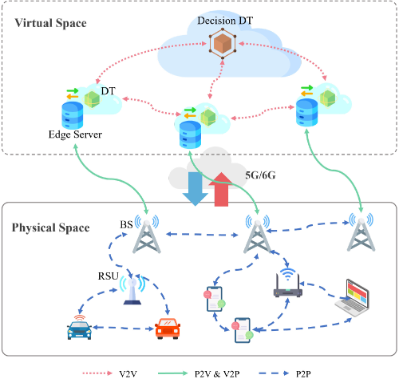
\includegraphics[width=0.3\linewidth]{figures/new_arch2.png}
        \caption{Artigos de arquitetura genérica de GD focam na infraestrutura de rede}
    \end{figure}
\end{frame}
\begin{frame}{Evolução de Arquitetura de GD}
\begin{figure}
        \centering
        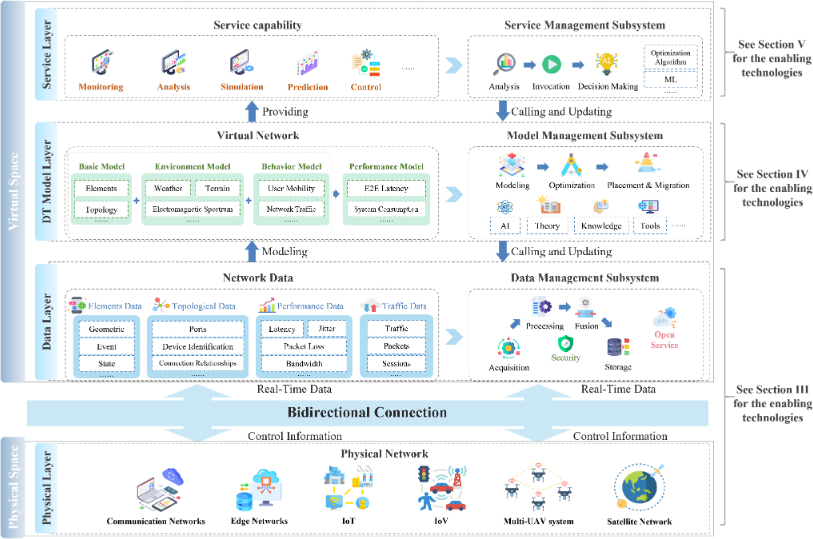
\includegraphics[width=0.9\linewidth, height=5cm]{figures/new_arch.png}
        \caption{Artigos de arquitetura genérica de GD focam na infraestrutura de rede}
    \end{figure}
\end{frame}


%------------------------------------------------
\section{Tipos dos Gêmeos Digitais}
%------------------------------------------------

\begin{frame}[plain]
    \vfill
    \centering
    {\Large\textcolor{dexpiBlue}{\textbf{Seção 3}}}\\[0.8em]
    {\LARGE\textbf{Tipos dos Gêmeos Digitais}}\\[0.6em]
    \vfill
\end{frame}

\begin{frame}{Tipos dos Gêmeos Digitais}
    Algumas classificações de Gêmeos Digitais (GDs):
    \vspace{0.4em}
    \centering
    \footnotesize
    \begin{tabular}{p{3.5cm}p{3.0cm}p{5.3cm}}
        \toprule
        \textbf{Foco} & \textbf{Pioneiros / Referência} & \textbf{Conceito Central} \\
        \midrule
        1. Ciclo de Vida & Grieves \cite{grieves2017dt} & DTP, DTI e DTA \\
        2. Fluxo de Dados & Kritzinger \cite{fuller2020dt} & Modelo, Sombra e Gêmeo Digital \\
        3. Granularidade & Vohra \cite{vohra2022dt} & Componente, Ativo, Sistema, Processo \\
        4. Cognitivos (CDT) & El Adl \cite{eladl2016cdt} / Zheng \cite{zheng2022emergence} & Raciocínio, Grafos de Conhecimento \\
        \bottomrule
    \end{tabular}
\end{frame}

\begin{frame}{As Dimensões da Cognição no Contexto do CDT}
    Proposto conceitualmente por Ahmed El Adl \cite{eladl2016cdt} e formalizado por Zheng et al. \cite{zheng2022emergence}, o CDT estende o gêmeo tradicional adicionando capacidades da mente humana \cite{alfaruque2021cdt} :
    \begin{columns}[T]
        \begin{column}{0.48\textwidth}
            \begin{block}{Interação e Filtro}
                \footnotesize
                \begin{itemize}\setlength\itemsep{0pt}
                    \item \textbf{Percepção:} Tradução de dados brutos de sensores em representações úteis.
                    \item \textbf{Atenção:} Foco computacional dinâmico em eventos e subsistemas em risco.
                \end{itemize}
            \end{block}
            \begin{block}{Retenção de Contexto}
                \footnotesize
                \begin{itemize}\setlength\itemsep{0pt}
                    \item \textbf{Memória:} Reter histórico (episódica), regras (semântica) e dados de trabalho.
                \end{itemize}
            \end{block}
        \end{column}
        \begin{column}{0.48\textwidth}
            \begin{block}{Processamento e Decisão}
                \footnotesize
                \begin{itemize}\setlength\itemsep{0pt}
                    \item \textbf{Raciocínio (\textit{Reasoning}):} Inferência lógica para deduzir diagnósticos explicáveis.
                    \item \textbf{Resolução de Problemas:} Geração autônoma de planos e ações corretivas.
                \end{itemize}
            \end{block}
            \begin{block}{Evolução}
                \footnotesize
                \begin{itemize}\setlength\itemsep{0pt}
                    \item \textbf{Aprendizado:} Evolução autônoma de modelos com novas experiências.
                \end{itemize}
            \end{block}
        \end{column}
    \end{columns}
\end{frame}

\begin{frame}{Comparativo: Digital Twin vs. Cognitive Digital Twin \cite{alfaruque2021cdt}}
    \centering
    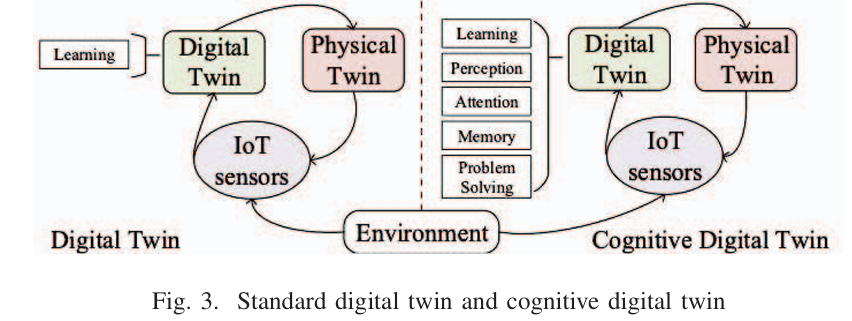
\includegraphics[height=0.55\textheight]{img/standard_vs_cognitive_digital_twin.png}
    \vspace{0.4em}
    \begin{itemize}
        \footnotesize
        \item \textbf{Digital Twin Tradicional (Esquerda):} Mapeamento físico-digital simples; a única inteligência é o aprendizado básico (\textit{Learning}) de padrões (Faruque[6]) .
        \item \textbf{Cognitive Digital Twin (Direita):} Dotado de um "cérebro" com múltiplas capacidades cognitivas integradas (Percepção, Atenção, Memória, Resolução de Problemas, Raciocínio) atuando sobre o ativo físico (faruque[6]).
    \end{itemize}
\end{frame}

\begin{frame}{Evolução do Volume de Publicações sobre CDTs}
    \begin{columns}[T]
        \begin{column}{0.52\textwidth}
            \centering
            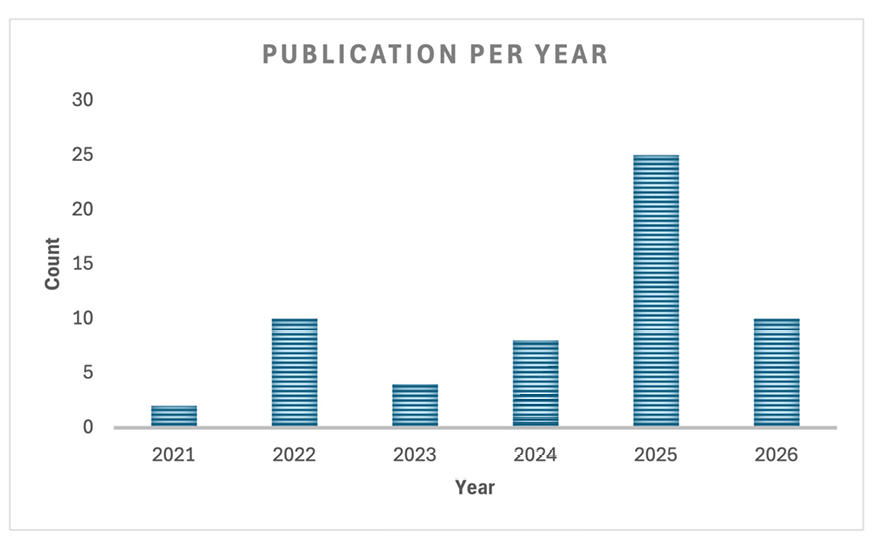
\includegraphics[width=\textwidth]{img/cdt_publications_per_year.png}
            \vspace{0.1em}
            \centerline{\tiny Distribuição de artigos por ano de publicação.}
        \end{column}
        \begin{column}{0.45\textwidth}
            \begin{block}{Metodologia de Contagem}
                \scriptsize
                Revisão sistemática (PRISMA 2020) conduzida nas bases **Scopus** e **Web of Science**.
            \end{block}
            \begin{block}{Critério de Alto Impacto}
                \scriptsize
                Inclui **apenas artigos de periódicos (*journals*)**. Capítulos de livros, conferências e editoriais foram excluídos.
            \end{block}
            \begin{block}{Conclusão da Tendência}
                \scriptsize
                Pico expressivo em 2025 (25 artigos), liderado pela área de **Manufatura (37\%)**.
            \end{block}
        \end{column}
    \end{columns}
    \vfill
    \footnotesize Fonte: Bacnak et al. \cite{bacnak2026systematic}.
\end{frame}

\begin{frame}{Casos de Sucesso do CDT em Operação}
    Aplicações práticas documentadas na literatura científica comprovam o valor dos CDTs:
    \vspace{0.4em}
    \begin{itemize}\setlength\itemsep{4pt}
        \item \textbf{Manufatura de Tubos de Aço \cite{zheng2022emergence}:} Um CDT de monitoramento mecânico utilizou aprendizado autônomo de vida útil dos componentes, gerando uma \textbf{redução de 10\% no consumo de energia} e minimizando paradas.
        \item \textbf{Montagem de Transmissões (PTU) \cite{zheng2022emergence}:} Integração de CDT com sensores heurísticos reduziu refugo industrial, elevando a precisão da detecção de falhas de montagem em \textbf{9\%}.
        \item \textbf{Prédios Inteligentes e Climatização (HVAC) \cite{elmokhtari2022hvac}:} Um CDT de controle preditivo realizou previsões de carga térmica 24 horas antes e ajustou dinamicamente ar-condicionado e luzes com base em presença, cortando desperdícios.
    \end{itemize}
\end{frame}


%------------------------------------------------
\section{Maior aprofundamento nos Exemplos}
%------------------------------------------------

\begin{frame}[plain]
    \vfill
    \centering
    {\Large\textcolor{dexpiBlue}{\textbf{Seção 4}}}\\[0.8em]
    {\LARGE\textbf{Maior Aprofundamento nos Exemplos}}\\[0.6em]
    \vfill
\end{frame}

\begin{frame}{A Origem do WIS (Well Integrity Surveillance)}
    \begin{alertblock}{Colapso do poço PW1}
        Uma operação não intencional despressurizou o anular A abaixo do limite de projeto, causando \textbf{colapso do revestimento} -- da superfície até a coluna de produção -- resultando em falha total e abandono do poço (Campos et al., 2019)
    \end{alertblock}
    \begin{itemize}
        \item \textbf{A descoberta veio dos dados}: simulando o comportamento do poço com os dados históricos, foi possível identificar o momento exato do colapso via modelagem matemática
        \item \textbf{Conclusão da Petrobras}: se a física explica a falha \textit{a posteriori}, um gêmeo digital rodando essa física \textbf{em tempo real} teria alertado antes do colapso
    \end{itemize}

    \vfill
    \footnotesize Incidente descrito em Campos et al. (2019) e retomado em \cite{otc2020}.
\end{frame}


\begin{frame}{Óleo e Gás -- WIS: Well Integrity Surveillance}
    \footnotesize
    \begin{itemize}
    \item O projeto de P\&D que evoluiu para o WIS -- avaliar em tempo real eventos críticos de integridade durante a produção
        \item \textbf{WIS (Well Integrity Surveillance)}: processo que integra um modelo de \textbf{escoamento transiente multifásico}  a um \textbf{modelo estrutural do poço} 
        \item Cargas calculadas \textbf{em tempo real} em função dos dados de produção (PDGs, árvore de natal, topside)
        \item Opera \textbf{24/7} em ambiente colaborativo: handover do poço, relatórios de inspeção/intervenção, dados de produção e modelagem de escoamento
    \end{itemize}
    
    \vfill
    \footnotesize Conteúdo baseado em \cite{spe210260,otc2020}.
\end{frame}

\begin{frame}{WIS -- Camada 1: Aquisição}
    \begin{itemize}\setlength\itemsep{6pt}
        \item Os \textbf{sensores do poço e da plataforma} são a base de tudo: sem dados de produção confiáveis e contínuos, não há como calcular cargas em tempo real
        \item Três fontes de dados de produção alimentam o twin: \textbf{PDGs} (sensores de fundo de poço), \textbf{árvore de natal} e \textbf{topside}
        \item Os dados são transmitidos em tempo real ao \textbf{Centro de Suporte}, onde o restante da arquitetura processa e interpreta essas séries
    \end{itemize}
    \begin{exampleblock}{Importância da Camada 1}
        Todas as camadas seguintes -- simulação, diagnóstico, decisão humana -- dependem da qualidade e da continuidade dos dados adquiridos aqui.
    \end{exampleblock}
    \vfill
    \footnotesize Conteúdo baseado em \cite{otc2020}.
\end{frame}

\begin{frame}{WIS -- Camada 2: Modelo Físico}
    \begin{itemize}\setlength\itemsep{5pt}
        \item Um \textbf{simulador de escoamento multifásico transiente} calcula o perfil de pressão e temperatura ao longo de todo o poço, a cada instante
        \item Esses perfis viram \textbf{cargas de entrada} do \textbf{modelo estrutural do poço}, que calcula:
        \begin{itemize}
            \item tensões nos revestimentos
            \item APB (\textit{Annulus Pressure Buildup}) nos anulares confinados
            \item fatores de segurança
        \end{itemize}
    \end{itemize}
    \begin{exampleblock}{O acoplamento termo-hidráulico $\rightarrow$ estrutural}
        É este acoplamento -- escoamento alimentando estrutura -- que transforma um simulador de fluxo comum em um digital twin de \textbf{integridade}: a física do fluido dentro do poço passa a ter sua dinâmica calculada em tempo real
    \end{exampleblock}
    \vfill
    \footnotesize Conteúdo baseado em \cite{otc2020}.
\end{frame}

\begin{frame}{WIS -- Camada 3: Diagnóstico}
    \begin{itemize}\setlength\itemsep{6pt}
        \item \textbf{Comparação contínua} entre o que é medido pelos sensores e o que o motor físico simula para aquele mesmo instante
        \item Divergências entre medido e simulado são o sinal de alerta: o sistema identifica automaticamente
        \begin{itemize}
            \item \textbf{washouts:} falha por erosão-corrosão acelerada que fura a parede de um tubo
            \item limites de \textbf{pressão/vazão} excedidos por equipamento
            \item falha de \textbf{DHSV (Downhole Safety Valve}
            \item \textbf{pack-off:} bloqueio ou obstrução total do espaço anular 
        \end{itemize}
    \end{itemize}
    \begin{exampleblock}{Acompanhamento Real-time}
        É esta camada que converte a réplica física em ferramenta de \textbf{diagnóstico}: o problema não precisa mais ser descoberto depois do fato -- ele aparece como desvio no momento em que ocorre
    \end{exampleblock}
    \vfill
    \footnotesize Conteúdo baseado em \cite{otc2020}.
\end{frame}

\begin{frame}{WIS -- Camada 4: Colaborativa/Humana}
    \begin{itemize}\setlength\itemsep{6pt}
        \item Vigilância \textbf{24/7} integrada a documentos operacionais: \textbf{handover} do poço, relatórios de \textbf{inspeção} e \textbf{intervenção}, dados de produção e modelagem de escoamento
        \item Engenheiros no centro de operações interpretam os alertas da camada de diagnóstico e decidem a ação.
    \end{itemize}
    \begin{exampleblock}{Validação em campo}
        Com essa arquitetura, a Petrobras implementou um \textbf{projeto piloto em três unidades de produção offshore} no Brasil, aumentando o conhecimento do comportamento estrutural do poço e, consequentemente, a segurança operacional dos ativos
    \end{exampleblock}
    \vfill
    \footnotesize Conteúdo baseado em \cite{otc2020}.
\end{frame}

\begin{frame}{Arquitetura Computacional}
\begin{center}
    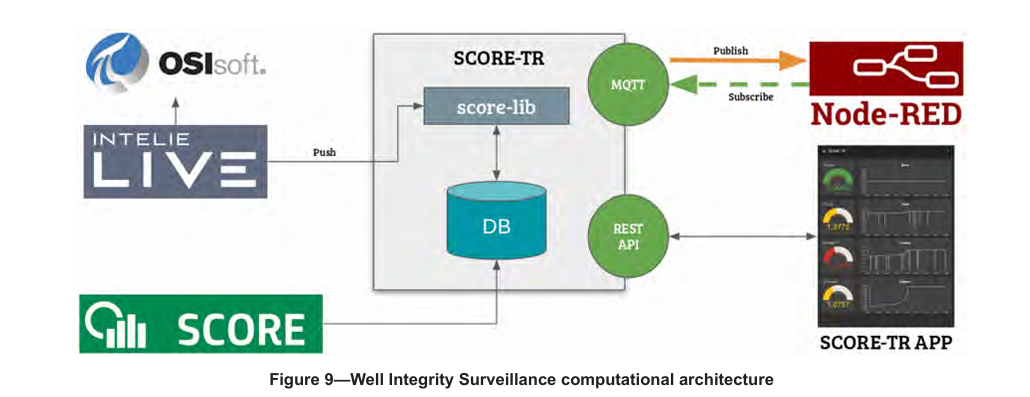
\includegraphics[
        height=0.6\paperheight,
        keepaspectratio
    ]{img/arquitetura_computacional.png}
\end{center}

\end{frame}


\begin{frame}

\begin{itemize}
    \item \textbf{Sensores → OSIsoft PI:} PDG, árvore de natal (TPT, válvulas) e topside gravam P, T e status no historian — só o anular A é medido; o anular B é calculado por pior caso
    \item \textbf{PI → WIS Live (Intelie):} a cada atualização, os dados são enviados ao motor de cálculo via publish/subscribe
    \item \textbf{SCORE-TR + score-lib:} Recebe os dados do poço e calcula os Fatores de Segurança mecânicos dinamicamente. Se o poço operar perto do limite físico de cargas, o SCORE-TR aciona um alarme crítico de integridade via WIS Live
    \item \textbf{Distribuição:} REST API + MQTT + Comet → dashboards, alertas e integração com Node-RED
\end{itemize}

\end{frame}

\begin{frame}{Monitoramento dos dados no Poço}
\begin{center}
    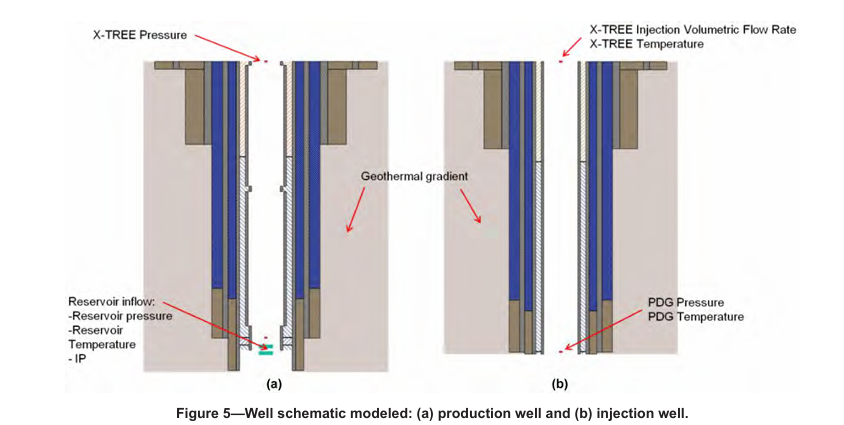
\includegraphics[
        height=0.7\paperheight,
        keepaspectratio
    ]{img/POÇO.png}
\end{center}

\end{frame}

\begin{frame}{Óleo e Gás -- WIS: Sensores e Dados Monitorados}
    \footnotesize
    O paper aponta três fontes de dados de produção:
    \begin{description}
        \item[PDG] \textit{\textbf{Permanent Downhole Gauge}} -- sensor permanente de fundo de poço (coluna de produção); mede \textbf{pressão e temperatura de fundo contínuas}, o dado mais valioso do poço. Ex.: uma operação inteira de interceptação de poço foi monitorada via PDG do PW1, permitindo identificar o momento exato da interceptação e deslocar os fluidos de cimentação com segurança
        \item[X-TREE] \textbf{árvore de natal molhada} -- pressão/temperatura na árvore (TPT), status de válvulas (WCT, DHSV) e métricas da linha de controle hidráulica do SCM, indicando a saúde hidráulica do sistema de controle submarino
        \item[Topside] \textbf{instrumentação da plataforma/FPSO} -- pressões, temperaturas e vazões de chegada, dados de separação e teste de poço
    \end{description}



    \vfill
    \footnotesize Palavras-chave do SPE-210260: \textit{pdg pressure}, \textit{pdg temp}. Conteúdo baseado em \cite{spe210260,otc2020}.
\end{frame}

\begin{frame}{Dashboard de Controle}
\begin{center}
    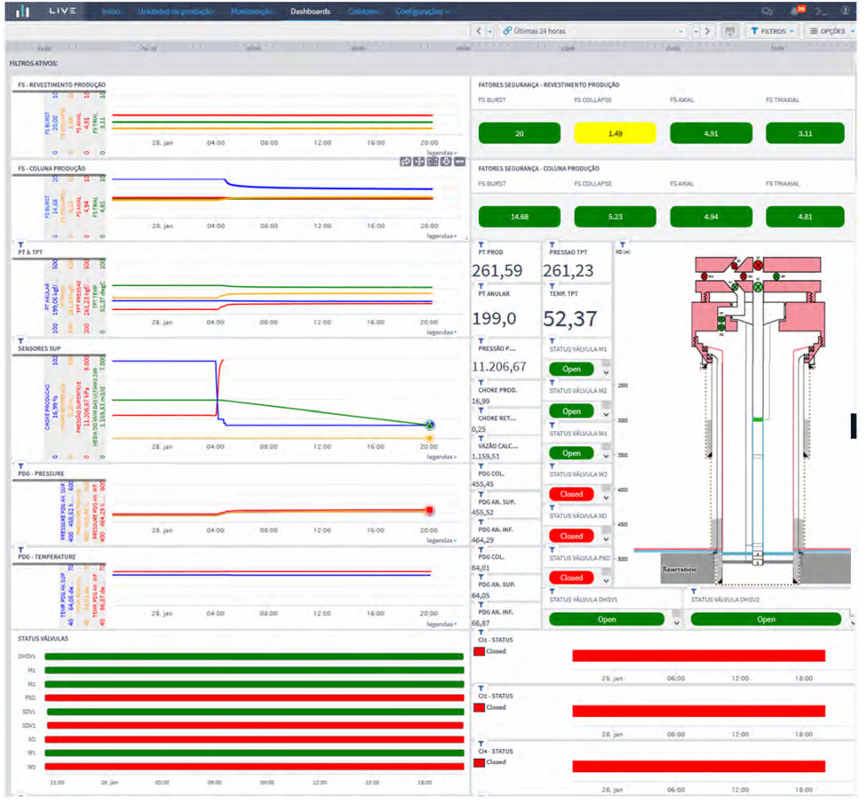
\includegraphics[
        height=0.7\paperheight,
        keepaspectratio
    ]{img/DASHBOARD.png}
\end{center}



\end{frame}






%------------------------------------------------
\section{Mais Benefícios}
%------------------------------------------------

% \begin{frame}[plain]
%     \vfill
%     \centering
%     {\Large\textcolor{dexpiBlue}{\textbf{Seção 4}}}\\[0.8em]
%     {\LARGE\textbf{Novos Exemplos}}\\[0.6em]
%     \vfill
% \end{frame}

\begin{frame}{5. Mais um benefício}

\vspace{0.2cm}

\begin{itemize}
    \item \textbf{Treinamento}: Além de usar o simulador para benchmarking e manutenção preditiva, facilita o treinamento de funcionários no controle de máquinas e situações de perigo. \cite{kaarlelaDTForSafetyTraining}
\end{itemize}

\vfill

\begin{center}
    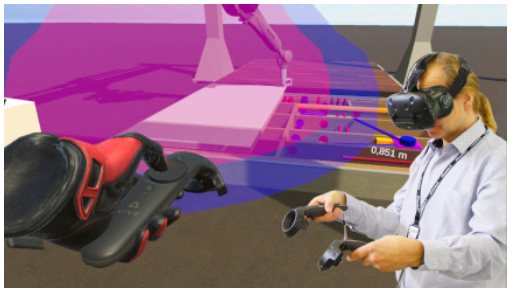
\includegraphics[
        height=0.4\paperheight,
        keepaspectratio
    ]{img/trainingVR.png}
    \hspace{0.5cm}
    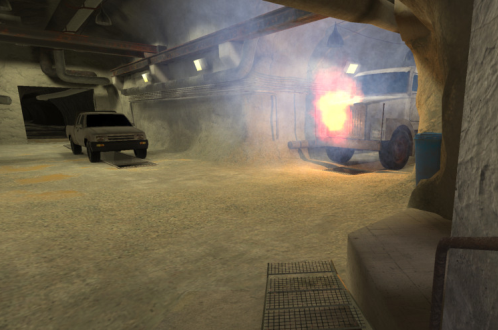
\includegraphics[
        height=0.4\paperheight,
        keepaspectratio
    ]{img/trainingFire.png}
\end{center}

\end{frame}


%------------------------------------------------
\section{Referências}
%------------------------------------------------

\begin{frame}[allowframebreaks]
\frametitle{Referências}
    \footnotesize
    \bibliographystyle{ieeetr}
    \bibliography{reference.bib}
    
\end{frame}

\begin{frame}
    \Huge{\centerline{\textbf{Chegamos ao Fim}}}
    \Huge{\centerline{\textbf{Obrigado pela sua Atenção}}}
\end{frame}


\end{document}